\section{Empirical Study}
\label{sec:case_study} 


For the validation of the proposed architecture we conducted an empirical study,
which consists of the evaluation of the main 
architectural decisions of SISDOT, which relate to the generation of QDMs.
The case study aims to answer the 
following research questions:

\begin{itemize}

% \item \textbf{RQ.1}: O uso da DSL na execução de testes reduz o esforço do profissional de testes durante a implementação dos casos de testes?
\item \textbf{RQ.1}: Does our proposed approach, based on meta-programming, generate correct QDMs?

\item \textbf{RQ.2}: Does the use of a DSL reduce the effort necessary to implement the test cases that target QDM generation? 

\item \textbf{RQ.3}: Does our proposed approach, based on meta-programming, generate QDMs within a satisfactory time-frame?

\end{itemize}

% A RQ.1 está relacionada à produtividade do testador e demonstra quanto código a menos o desenvolvedor deve implementar ao utilizar a DSL criada, em comparação com a declaração do mesmo chamador utilizando a linguagem Java. Apesar de não haver formalmente um requisito funcional especificando qual seria um tempo aceitável para a geração de um QDM, foi determinado que um tempo maior que 5 segundos, ao utilizar 1000 chamadores, é inaceitável. Assim, a RQ.2 serve para garantir que os QDMs sejam gerados em tempo satisfatório.

\textbf{RQ.1} deals with the most important concern: correctness regarding the QDM generation. It is intended 
to demonstrate that the solution not only automatically generates the rules, eliminating the work that the developer 
would have to implement the solution in Java, but also that the proposed approach leads to the expected QDMs when considering 
a well defined set of \callers.
\textbf{RQ.2} is related to the productivity of the tester and demonstrates how much code the 
developer have to write when using our DSL, compared to the effort to specify \callers using the Java language in 
unit test cases. During the activities of requirements elicitation,
we identified a softgoal stating the  acceptable time for generating a QDM, 
which should not be above 5 seconds, when using 1000 \callers.
Thus, \textbf{RQ.3} serves to ensure that the QDMs are generated in a satisfactory time.

% Com a RQ.3 pretende-se demonstrar que a solução gera as regras automaticamente, eliminando o trabalho que o desenvolvedor teria para implementar a solução em Java. Com poucas linhas de código, relacionadas à definição do template e sua execução, a solução gera um arquivo de regras com determinado número de linhas de código Drools. A resposta dessa questão está relacionada aos resultados dos testes manuais e automáticos.


\subsection{Data Collection and Analysis Procedures}

% A coleta dos dados foi realizada utilizando as seguintes métricas: linhas de código (LOC) e tempo de execução. A escolha dessas duas métricas está relacionada ao tamanho do código, que pode indicar uma maior produtividade; e à satisfação do requisito funcional que determina o tempo máximo de execução para a geração de QDM. 
We answer our first question qualitatively. Although this might look like disappointing (under the 
perspective of empirical methods), we have strong evidences collected from the domain experts 
that our approach has produced correct QDMs. We believe that this correctness is due to several 
factors, including the involvement of the domain experts that helped us to full understand 
the requirements and the expertise of our development team. Nevertheless, the decision of 
not writing the low-level rules at the source code level, but instead using a program 
generation approach that has reduced significantly the effort needed to \emph{hand write} 
those rules, has also contributed to achieve this confidence about correctness. 

In a meeting 
with the domain experts, one of the specialists said: ``I got surprised with the 
correctness of the solution. In the previous version of the system, we had to have several 
interactions until we got confident about the correct operation of the \callers''. The first 
time that we generate QDMs, the process was validated. It is important to note that ``not all 
are flowers'', and we broke the initial implementation after the introduction of a new, 
at first not so related feature that, in the end, cut across several classes of 
the system. We fixed the related issues recently.  

To answer the other two research questions, we collected the following metrics: lines of code (LOC) and execution time. The choice of these 
two metrics is related to the size of the code, which may indicate higher productivity; and to the fulfillment of the 
functional requirement that determines the maximum execution time for the generation of QDMs.

%A Tabela \ref{table:comparacao} apresenta a comparação dos resultados obtidos utilizando DSL e Java. 

\begin{table}[htb!]
\centering
\caption{Comparing the number of lines of code need to specify test cases using our DSL and Java}
\label{table:comparacao}
\begin{center}
\begin{tabular}{ccc}
\toprule
\textbf{\shc Code} & \textbf{Lines of Code (DSL)} & \textbf{Lines of Code (Java)}     \\ \midrule
1        & 10  & 26   \\ % \hline
2        & 10  & 25   \\ % \hline
3        & 10  & 32   \\ % \hline
4        & 11  & 52   \\ % \hline
5        & 15  & 41   \\ % \hline
6        & 9   & 16   \\ % \hline
7        & 18  & 21   \\ % \hline
8        & 12  & 25   \\ % \hline
15       & 7   & 45   \\ % \hline
58       & 7   & 58   \\ % \hline
59       & 17  & 34   \\ \bottomrule
\end{tabular}
\end{center}
\end{table}

% No cenário de testes considerado para o estudo de caso, o sistema SISDOT possuia  66 chamadores declarados em sua base de dados. Esses chamadores correspondem a chamadores reais utilizados pelo Exército Brasileiro (EB) para a realização de alguns testes na geração de QDMs. A conversão de cada chamador escrito na linguagem Java para o seu correspondente no formato da DSL foi realizada com o uso do Xtext. A Table \ref{table:comparacao} apresenta uma amostra dos dados coletados. A primeira coluna contém o código do chamador, a segunda coluna contém a quantidade de linhas de código para representar o chamador na DSL e a terceira coluna contém a quantidade de linhas para representar o mesmo chamador na linguagem Java.

We use as a benchmark 66 \callers declared in its database. These \callers correspond to real rules used by 
the Brazilian Army to perform some tests related to the generation of QDMs. We converted  
each \shc written using JUnit to their correspondent one specified using our DSL. 
Table \ref{table:comparacao} presents a sample of the collected data. The first column contains 
the \shc code, the second column contains the number of lines of code to represent the \shc using our DSL, and the third 
column contains the number of lines of code to represent the same rule in the Java language.

% Para a coleta da métrica de tempo de execução foi utilizado um computador com processador Intel(R) Core(TM) i7-4790, com 16GB de memória RAM, com o sistema operacional Ubuntu 16.04.4 LTS, 64 bits, com kernel 4.15.0-24-generic. Foram usados 16 QCs, escolhidos de forma a representar os variados tipos de OM, naturezas e subnaturezas. Para cada QC foram gerados QDMs usando as seguintes quantidades de chamadores: 20, 40, 50, 60, 100, 200, 400, 700, 1000, 1500, 2000, 3000, 5000. Como só haviam 66 chamadores reais já declarados, os conjuntos com quantidade maior contém chamadores repetidos. A seleção dos chamadores foi realizada de maneira randômica, mas com o mesmo seed, para que os mesmos conjuntos fossem utilizados nas gerações dos QDMs de diferentes QCs. A Table \ref{table:tempo} apresenta uma amostra dos resultados obtidos com a execução. A primeira coluna contém o código do QC, e da segunda coluna em diante contém o tempo, em milisegundos, para a geração dos QDMs usando a quantidade de chamadores indicada no header da respectiva coluna.

Regarding the runtime metrics, we collected the data using an Intel(R) Core{TM} i7-4790 processor, 
with 16GB of RAM, running Ubuntu 16.04.4 LTS 64-bit operating system, with 4.15.0-24-generic kernel. We used 16 QCs, 
chosen to represent the various OM types, natures, and sub-natures. For each QC, we generated QDMs using 
random sets of \callers with size: 20, 40, 50, 60, 100, 200, 400, 700, 1000, 1500, 2000. 
Since there were only 66 real \callers already declared, larger quantities contain repeated \callers (which in the end will duplicate 
the data within a given QDM). The selection of \callers was performed at random, but with the same seed, so that the same sets were used in the 
generation of QDMs for different QCs. Table \ref{table:tempo} shows a sample of the results obtained with the execution. 
The first column contains the QC code, and the second column contains the time in milliseconds for the generation of 
the QDMs using the indicated amount of \callers on the respective column header.

\begin{table}[htb!]
\centering
\caption{Time (ms) for generation of QDMs}
\label{table:tempo}
\begin{center}
\begin{tabular}{lllllll}
\toprule
\textbf{QC}      & \textbf{60}  & \textbf{100} & \textbf{400}  & \textbf{700}  & \textbf{1000} & \textbf{2000} \\ \midrule

206410  & 184 & 275 & 944  & 1829 & 2279 & 4707 \\ % \hline
231303  & 197 & 282 & 975  & 1731 & 2541 & 4987 \\ % \hline
500311  & 201 & 291 & 948  & 1804 & 2289 & 4950 \\ % \hline
618322  & 175 & 264 & 922  & 1640 & 2412 & 4990 \\ % \hline
727310  & 173 & 302 & 937  & 1652 & 2466 & 4992 \\ % \hline
1450311 & 182 & 269 & 890  & 1649 & 2527 & 4785 \\ % \hline
2203310 & 197 & 263 & 909  & 1619 & 2344 & 4976 \\ % \hline
5406194 & 176 & 253 & 884  & 1598 & 2393 & 4610 \\ % \hline
7020003 & 212 & 241 & 922  & 1610 & 2361 & 4470 \\ % \hline
9131000 & 171 & 252 & 888  & 1609 & 2345 & 4471 \\ \bottomrule
\end{tabular}
\end{center}
\end{table}

We exported the collected data to the CSV format, so that we could perform a data analysis using the R environment~\cite{crawley2013}. 
In the data analysis for \textbf{RQ.2}, which compares the number of lines of code between the two distinct approaches for 
representing \callers, we created two additional columns: \emph{difference}, which measures the difference in the number of 
lines of code necessary to specify \callers using Java and our DSL; and \emph{percent of reduction}, which indicates 
how much less code is necessary to specify a \shc using our DSL, when compared to the direct specification in Java code.

\begin{table}[htb!]
\centering
\caption{Analysis of DSL and Java comparison data}
\label{table:analiseComparacao}
\begin{center}
\begin{tabular}{llllll}
\toprule
           & \textbf{Min.}  & \textbf{Median} & \textbf{Mean}  & \textbf{SD}    & \textbf{Max.}  \\ \midrule
DSL        & 7.00  & 9.00   & 9.67  & 2.81  & 18.00 \\ % \hline
Java       & 9.00  & 17.50  & 21.76 & 14.68 & 96.00 \\ % \hline
Difference & 2.00  & 7.00   & 12.09 & 13.94 & 83.00 \\ % \hline
\%         & 14.29 & 43.75  & 45.23 & 19.84 & 87.93 \\ \bottomrule
\end{tabular}
\end{center}
\end{table}

% Na Table \ref{table:analiseComparacao} é possível observar algumas estatísticas descritivas dos dados coletados, contendo as seguintes colunas: valor mínimo, mediana, média, desvio padrão e valor máximo. Existe uma forte correlação entre as colunas Java e Difference, de 0.982. Essa correlação pode ser visualizada na Figure \ref{fig:correlacao}. É possível identificar que a medida que o tamanho do código Java cresce a diferença para a representação em DSL também aumenta. 

Table \ref{table:analiseComparacao} presents some descriptive statistics 
of the collected data, containing the following columns: minimum value, median, mean, standard deviation, and maximum value. 
There is a strong correlation (0.982) between the lines of code in Java and the \emph{difference} measurements. 
This correlation can be seen in Figure \ref{fig:correlacao}. It is possible to identify that as the size of the Java code grows, 
the difference for the representation in DSL also increases.

\begin{figure}[htb!] 
\centering
  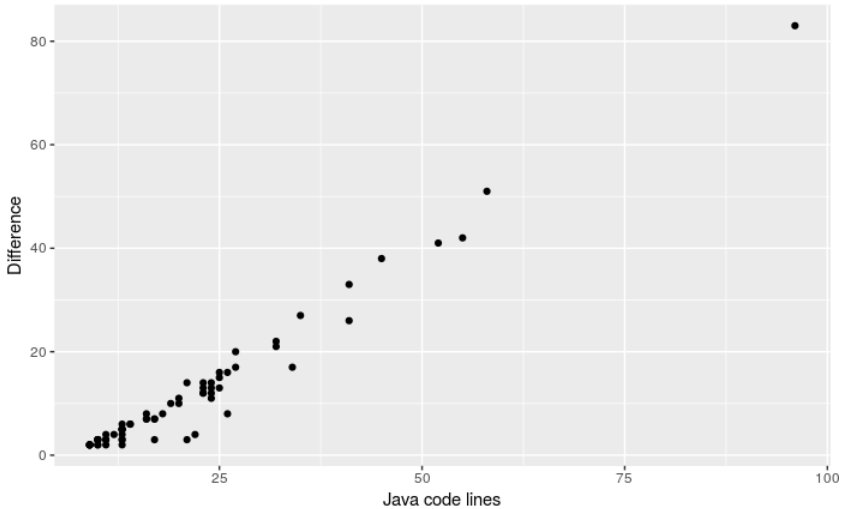
\includegraphics[width=.48\textwidth]
  {img/artigo_correlacao.jpg}
  \caption{\it Correlation between Java and Difference}
  \label{fig:correlacao}
\end{figure}

Figure \ref{fig:geracao} shows the time necessary to generate QDMs for 5 different QCs. For each of them, 
6 QMS were generated, with different amounts of \callers, 60, 100, 400, 700, 1000 and 2000.

\begin{figure}[!ht] \centering
  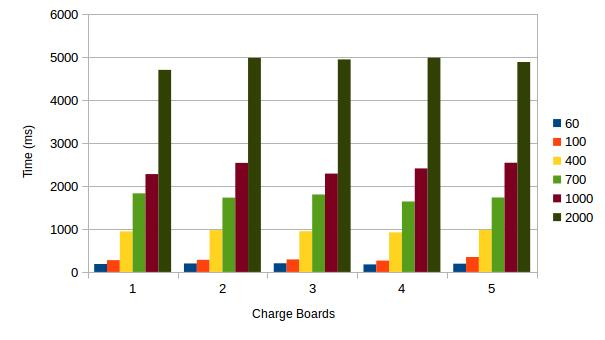
\includegraphics[width=.48\textwidth]
  {img/artigo_geracao.jpg}
  \caption{\it QDM Generation Time (ms)}
  \label{fig:geracao}
\end{figure}

\subsection{Discussion, Lessons Learned, and Threats to Validity}

When analyzing the data related to RQ.2, it was possible to realize that the representation 
of a \shc using our DSL is on average 45\% smaller than the representation of the same rule in Java. 
This indicates a possible productivity gain for the developer when writing test cases, 
since her will have to write a smaller amount of code. In addition, using our DSL, we 
specify \callers using a declarative approach, which is close to the vocabulary of 
the problem domain. With respect to the third research question, the limit imposed by the
functional requirement of 5 seconds was not exceeded, even when considering 2000 \callers,
which is twice the number of \callers expected for the system in production. It is important
to notice that these number (5 seconds as time limit and 1000 \callers were collected together
with the stakeholders of SISDOT).

The general approach discussed in this paper involves the use of metaprogramming
to generate low-level Drools rules from \callers and the use of a DSL to specify
\callers during test activities. We have some previous experience using Drools,
and, at the beginning of this research collaboration, we realized that the use of
a rule based engine (such as Drools), could simplify the computation of QDMs
(one of the main products of SISDOT). Nevertheless, we should try to abstract
the use of Drools, mostly due to architectural conformance---we should not
introduce new languages during the development of SISDOT. For this reason, we applied a
transformational approach, translating Java domain objects into
Drools rules at runtime. Perhaps due to the structure of the \callers, the task of implementing
this transformational approach was not difficult. We believe that it was the
right decision considering the original set of requirements. Surely, a number of uncertainties arise,
including: ``will our proposed approach support
the expectations of the end-users w.r.t. correctness
and time constraints?''. We address this question in our empirical evaluation.

However, we found that testing the process of QDM generation was
time consuming, and then we designed a DSL to address the main
bottleneck: the specification of \callers either using Java test scripts
or the SISDOT user interface (the common way for specifying \callers). Our choice
for using Xtext to this end had simplified the entire process for
implementing a DSL. Even considering that \hlrdsl is a simple and
small DSL, we argue that the set of Xtext tools is really simple and productive,
reducing the overall effort to implement the \hlrdsl grammar, parser, and
program generator. We could have used other tools and techniques as well, for instance
a metaprogramming approach to support our test activities. However,
such approach would not have solved the main problem that motivated us
to implement \hlrdsl. In this case, our goal was to design a simple
approach for specifying \callers. In the end, \hlrdsl started to
be considered an interesting approach for use not only in test
activities, but also for simulating QDMs without the need
to persist \callers in the production environment. 



% Foram usados apenas 66 chamadores reais, que serviram de base para medir o tempo de geração de QDMs. Espera-se que o SISDOT tenha por volta de 1000 chamadores, quando o mesmo estiver em ambiente de produção. Apesar da pequena quantidade de chamadores utilizada, incluindo suas repetições quando necessário, é esperado que o sistema cumpra o requisito funcional, pois os testes com o dobro de chamadores esperados ainda estão dentro do tempo máximo aceitável de 5 segundos para geração de QDM.

Our empirical study presents several limitations. First, we discuss
\emph{correctness} based on the results of both integration and acceptance
tests, though also considering the opinion of the domain experts that are
currently confident that our approach for QDM generation is working
properly. Surely, we could have used a more formal approach for
discussing correctness, and we postpone this investigation to a future
work. Nevertheless, considering the scope of this paper, the feedback
from the domain experts and testing outcomes reduce some of ours
uncertainties about correctness. 


Second, we only considered 66 real \callers in our study, which served as a basis
for measuring the time to generate QDMs. SISDOT is expected to have around 1000
\callers in the production environment. To mitigate the threat 
related to the small number of available \callers for testing, we considered their repetition
when carrying out a performance test of SISDOT. In this way, we expect that the
system would present a behavior similar to the production environment (with respect to performance).
The same situation occurs with the comparison of lines of code between the declarations
of \callers in DSL and Java. As the number of \callers is relatively small, 
it may not be possible to generalize the results we found.
